\documentclass[11pt]{article}
\usepackage[left=0.85in,right=0.85in,top=1in,bottom=1in]{geometry}
\usepackage[T1]{fontenc}
\usepackage[utf8]{inputenc}
\usepackage{lmodern}
\usepackage{amsmath,amssymb,booktabs}
\usepackage{graphicx,longtable}
\usepackage[numbers,sort&compress]{natbib}
\usepackage[hidelinks]{hyperref}
\usepackage{url}
\setlength{\emergencystretch}{1em}
\renewcommand{\topfraction}{0.9}
\renewcommand{\bottomfraction}{0.85}
\renewcommand{\textfraction}{0.10}
\renewcommand{\floatpagefraction}{0.8}

% Venue-neutral complete empirical draft; conference/template not yet selected.
% Full-revision input HEAD: 56ab6cee930da08637c3fa7c6b36d5cb22ccf09f.
% Experiments permanently frozen. Never alter research/final_evidence/.
% Recommended title below; alternatives:
% - Controlled Evidence on Distillability in Warm-Start Language Modeling
% - Teacher Quality and Distillability in Warm-Start Language Modeling
% TODO[VENUE]: research lead chooses venue before template/page-limit binding.
% TODO[AUTHOR]: insert approved authors/affiliations only at full writing stage.
\title{What Makes Knowledge Distillation Transfer?\newline
Controlled Evidence from Warm-Start Language Modeling}
\author{Anonymous authors}
\date{}

\begin{document}
\maketitle
\begin{abstract}
Knowledge distillation (KD) is commonly evaluated by the performance of the distilled student, yet a more basic question is often left implicit: given an already trained student, does adding teacher supervision actually improve over continuing maximum-likelihood training from the same state? We study this question in autoregressive language modeling using matched warm-start continuations, controlled teacher interventions, and independent student replications. Under the same token-normalized KD formulation, KD yields reproducible positive transfer on Penn Treebank and WikiText-2 but reproducible negative transfer on TinyStories, with consistent directions across three student initializations in each setting. We then test several natural explanations for these outcomes. At fixed teacher architecture and fusion composition, changing the trained teacher state reverses the sign of transfer, showing that teacher state and predictive quality strongly modulate distillation. However, global teacher likelihood is not sufficient: a teacher that is worse than the matched student on held-out likelihood still improves all three students. Likewise, greater branch disagreement and architectural heterogeneity do not imply better transfer; a homogeneous Transformer ensemble outperforms the heterogeneous Transformer--Grassmann teacher in all three matched comparisons. Additional local gradient and curvature diagnostics also fail to reliably predict long-horizon transfer. Together, these results support a configuration-dependent view of distillability: whether KD helps depends jointly on the teacher, the warm-start student, and the training configuration, and is not captured by a single teacher-quality or compatibility statistic.
% TODO[ABSTRACT:C1-C4]: paired +/+/- transfer; fixed-composition state reversal;
% weaker-source counterexample; homogeneous ensemble falsification.
% MUST NOT: method/geometry superiority; universal diagnostic; clean modern KD.
\end{abstract}

\section{Introduction}\label{sec:introduction}
\writingtodo{Introduce the paired warm-start distillation question and C1--C4.}
% - RQ: what determines useful transfer to an already-trained LM student?
% - C1/E1-E3: PTB/WT2/TinyStories gains +0.144937/+0.155665/-0.107219,
%   three independent student seeds each, not dataset-caused sign.
% - C2/E4: fixed alpha0.5 J/A state intervention, Q +0.183319 NLL.
% - C3/E5: globally weaker G versus C0, yet gain +0.040991.
% - C4/E6-E7: fused > branches; TT > TG, H -0.012460, caveats retained.
% TODO[CITE]: teacher accuracy insufficiency is not new; use cho2019efficacy,
% kaplun2022bad and closest autoregressive prior zhong2024atkd.
% TODO[NOVELTY]: specific controlled evidence chain, no new loss/theory.
% MUST NOT: old Grassmann-specific contribution, first harmful LM KD,
% universal teacher selection rule or clean modern-scale abstract headline.

\section{Related Work}\label{sec:related-work}
\writingtodo{Write from the overlap audit after closest-paper full-text checks.}
% - Teacher quality / student-oriented teachers: cho2019efficacy,
%   park2021friendly, menon2021statistical, kaplun2022bad.
% - Selection / compatibility: yuan2021selection, zhou2022metadistil.
% - Autoregressive adaptive KD: zhong2024atkd is the closest direct prior;
%   gu2024minillm, agarwal2024gkd, xie2026adakd concern established loss/state
%   and student-distribution issues; jin2026entropy concerns uncertainty.
% - Ensemble / gradient-aware / validation-driven: stanton2021really,
%   du2020agree, zhou2022metadistil.
% - Harmful supervision: wang2021selective, zhong2024atkd.
% TODO[FULLTEXT]: verify initialization/CE comparators/checkpoint selection
% before asserting a protocol distinction; abstracts do not prove absence.
% TODO[CITE:VERIFY_EXTERNAL]: foundational KD, Transformer/Grassmann,
% PTB/WT2/TinyStories/FineWeb-Edu/SmolLM2 primary dataset/model citations.
% MUST NOT: invent bibliography entries or claim superiority over these
% adaptive methods, since none was run as a comparison in this study.

\section{Problem Setting and Paired Distillability Evaluation}
\label{sec:problem-setting}
\writingtodo{Specify the operational gain and matched checkpoint-selection unit.}
% - Gain = test_NLL_CE - test_NLL_KD; positive means benefit over matched CE.
% - Same S0 hash within each seed, independent student preparations between
%   seeds; frozen teacher; validation-NLL selects, test only reports endpoints.
% - Existing token_mean forward KL(p_T || p_S), T=2, archived T^2 scaling.
% TODO[LOSS]: transcribe implementation normalization exactly, not legacy
% batchmean; state target mask/shift and finite optimizer reset protocol.
% - Three paired-gain sample SDs are not SEs or significance tests.
% - Phase4B primary excludes S0; best_including_S0 is separate diagnostic;
%   Phase4C includes S0 in CE gate, has no authorized KD/test after failure.
% MUST NOT: definition-as-theorem, unmatched random-init necessity proof.
\figureplaceholder{F1: Paired warm-start evaluation}
{Exact S0 forks into matched CE and KD; independent validation selection;
final test reporting. Step-0 eligibility is a separately labeled protocol choice.}
{fig:paired_protocol}

\section{Teacher Construction and Controlled Interventions}
\label{sec:experimental-setting}

The primary test bed comprises PTB~\citep{marcus1993ptb}, WikiText-2~\citep{merity2016wikitext}, and TinyStories~\citep{eldan2023tinystories}. Small models use the same local GPT-2 tokenizer and sequence length 256. Within each corpus, independently prepared students undergo matched 10-epoch CE and KD continuations. Corpus sizes, frozen teachers, and preparation histories differ across domains, so paired gains, rather than absolute cross-domain NLL, are the comparable quantities. Appendix~\ref{app:protocols} specifies the archived configurations and checkpoint identities.

Our heterogeneous teacher combines a Transformer branch~\citep{vaswani2017attention} and a causal Grassmann branch by late-logit fusion:
\begin{equation}
z_{\mathrm{TG}}=\alpha z^{(\mathrm{T})}+(1-\alpha)z^{(\mathrm{G})}.
\label{eq:teacher-fusion}
\end{equation}
Fusion is applied before softmax, not to branch probabilities. The Grassmann branch supplies a structurally different supervision source in an existing test bed, rather than a new method contribution. Its causal local-pair processing and feature-dependent gate are specified in Appendix~\ref{app:architecture}.

The fixed-composition teacher-state intervention compares two WikiText-2 checkpoints with the same architecture and source identities. Teacher J was jointly trained; Teacher A updated only the fusion weight while keeping source branches frozen. Both use $\alpha=0.5$ for evaluation and KD. The intervention therefore changes trained parameter states, including branch representations, without changing fusion composition. The source ablation instead holds Teacher J fixed and sets $\alpha$ to 0.5, 1, or 0 for fused, Transformer-only, or Grassmann-only supervision.

The homogeneous ensemble control adds a second independently trained Transformer, matching the existing source architecture, data, tokenizer, and 20-epoch preparation budget. Subsequent joint training follows the 10-epoch teacher schedule with branches frozen in the first epoch. Both TT and TG use $\alpha=0.5$ for evaluation and KD. Their teacher training histories, fusion-weight learning rates, predictive quality, and parameter counts are not identical; these differences constrain interpretation.

Teacher quality is measured on a fixed 512-chunk validation subset with 130,560 targets for the state and source analyses, but on full validation for TT/TG. These scopes remain separate. WikiText-2 controls reuse the same CE and TG student endpoints, not additional independent replications. A retrospective diagnostic tests local predictors without new training, while a separate pretrained-model stress test examines modern continuation. Neither is pooled with primary cross-domain evidence.

\section{Reproducible Positive and Negative Transfer}
\label{sec:cross-domain-transfer}

Table~\ref{tab:cross_domain_transfer} reports the matched three-seed comparisons. Warm-start KD improves PTB test NLL by $0.144937\pm0.003938$ and WikiText-2 by $0.155665\pm0.007692$ (mean $\pm$ sample SD). The corresponding mean CE and KD NLLs are 4.082352 and 3.937415 on PTB, and 4.276364 and 4.120699 on WikiText-2. Every paired gain is positive in both domains.

TinyStories exhibits the opposite direction. Mean test NLL increases from 1.582197 under CE to 1.689416 under KD, yielding a gain of $-0.107219\pm0.000415$. All three independently prepared students are harmed relative to matched CE continuation. Figure~\ref{fig:cross_domain_gain} places these paired gains on the same sign convention.

In these small-model TinyStories runs, CE improves over $S_0$ on test for every seed, unlike the modern continuation regime discussed in Section~\ref{sec:external-validity}. All accepted endpoints are finite. KD nevertheless has higher mean gradient norms and clipping fractions of 0.237--0.283, compared with 0.000391 for CE; maximum AMP overflow/nonfinite fractions are 0.000611 and 0.000488, respectively. The negative result is therefore specific to the frozen optimization protocol, not an optimization-independent property of KD. An incomplete, power-capped seed-456 attempt was excluded; its authorized, protocol-identical restart from scratch is the accepted endpoint (Appendix~\ref{app:protocols}).

The positive--positive--negative pattern establishes that this token-normalized warm-start KD recipe has no uniform transfer effect across the tested configurations. It does not identify the cause of the sign change: teacher state, student preparation, and corpus properties vary jointly across domains. The controlled analyses that follow investigate candidate explanations within WikiText-2. Unmatched legacy results, including single-seed observations with batch-normalized KL, are excluded from this confirmatory comparison.

% Generated from frozen sources by build_tables.py; not a prose draft.
\begin{table}[htbp]
\centering\small
\begin{tabular}{lrrrr}
\toprule
Dataset & CE NLL & KD NLL & Gain (mean $\pm$ SD) & Signs \\
\midrule
PTB & 4.082352 & 3.937415 & 0.144937 $\pm$ 0.003938 & 3/3 + \\
WikiText-2 & 4.276364 & 4.120699 & 0.155665 $\pm$ 0.007692 & 3/3 + \\
TinyStories & 1.582197 & 1.689416 & -0.107219 $\pm$ 0.000415 & 3/3 -- \\
\bottomrule
\end{tabular}
\caption{Paired warm-start transfer across three text domains (planning table).}
\label{tab:cross_domain_transfer}
\par\smallskip\begin{minipage}{0.96\linewidth}\footnotesize Three independently trained student initializations per dataset; one frozen teacher per dataset. Gain is CE minus KD test NLL. Sample SD is over paired gains, not an SE. $\lambda=5$, $T=2$, token-mean KD; validation-selected endpoints. Cross-domain comparisons do not isolate a causal dataset effect.\end{minipage}
\end{table}

\figureplaceholder{F2: Cross-domain paired transfer}
{Per-seed CE-relative NLL gain on PTB, WikiText-2, and TinyStories;
mean and sample SD over three independent student preparations per domain.}
{fig:cross_domain_gain}

\section{What Determines Teacher Distillability?}
\label{sec:distillability}

\subsection{Fixed-composition teacher-state intervention}
\label{sec:teacher-state}

To separate teacher state from composition, we compare jointly trained Teacher J with fusion-weight-only Teacher A at the same $\alpha=0.5$. Their teacher validation-subset NLLs are 4.300644 and 6.376220. Teacher J produces positive transfer in all three students, whereas Teacher A produces negative transfer in all three: mean gains are $+0.155665\pm0.007692$ and $-0.027654\pm0.006822$ (Table~\ref{tab:teacher_state}). The paired state contrast is
\begin{equation}
Q=\mathrm{NLL}_{\mathrm{KD,A}}-\mathrm{NLL}_{\mathrm{KD,J}}
=+0.183319\pm0.001375,
\label{eq:teacher-state-contrast}
\end{equation}
with all three differences positive.

The reversal shows that teacher training state matters even with fixed architecture and fusion composition. It does not isolate scalar likelihood as the cause: joint training also changes branch representations and the distribution of errors. Better predictive quality accompanies more useful supervision here, but the intervention is on trained teacher state, not NLL alone. Optimization gates and the documented protocol amendment are retained in Appendix~\ref{app:protocols}.

\subsection{A globally weaker teacher can still help}
\label{sec:weaker-teacher}

The Grassmann-only source supplies a counterexample to a simple likelihood rule. Its validation-subset NLL is 4.652064, worse than every matched CE endpoint on that subset, yet its test gain is positive in all three students, averaging $+0.040991\pm0.006733$ (Table~\ref{tab:weaker_teacher}). A globally weaker teacher can therefore provide useful supervision under this continuation protocol.

The reference student is the validation-selected CE continuation, not an arbitrary initialization. Teacher residual advantage and transfer gain also use different held-out scopes, as stated in the table. This result does not make teacher quality irrelevant; together with the state reversal, it shows that global held-out teacher likelihood alone is insufficient to determine distillability. Figure~\ref{fig:teacher_quality} summarizes these complementary controls without assigning a geometric cause to the gain.

% Numeric rows formatted from frozen archived tables; caption revised 2026-10-08.
\begin{table}[htbp]
\centering\small
\begin{tabular}{lrrrr}
\toprule
Teacher/state contrast & Teacher val NLL & Gain/contrast & Sample SD & Signs \\
\midrule
Joint J & 4.300644 & 0.155665 & 0.007692 & 3/3 + \\
Alpha-only A & 6.376220 & -0.027654 & 0.006822 & 3/3 -- \\
$Q$ (student test contrast) & -- & 0.183319 & 0.001375 & 3/3 + \\
\bottomrule
\end{tabular}
\caption{Fixed-composition teacher-state intervention on WikiText-2. Teacher NLL uses the same 512-chunk validation subset; gains are CE-relative test endpoints over three students. $Q$ compares A with J within a student. Composition is fixed, but trained representations differ.}
\label{tab:teacher_state}
\end{table}

% Generated from frozen sources by build_tables.py; not a prose draft.
\begin{table}[htbp]
\centering\small
\begin{tabular}{lrr}
\toprule
Seed & Teacher residual vs C0 & KD test gain \\
\midrule
42 & -0.266520 & 0.046771 \\
123 & -0.253492 & 0.033598 \\
456 & -0.251006 & 0.042604 \\
\bottomrule
\end{tabular}
\caption{A globally weaker teacher can still transfer positively (planning table).}
\label{tab:weaker_teacher}
\par\smallskip\begin{minipage}{0.96\linewidth}\footnotesize Residual is C0 validation-subset NLL minus teacher NLL. All residuals are negative while gains are positive. This refutes a universal necessity rule; it does not show that weak teachers are usually better or that likelihood is irrelevant.\end{minipage}
\end{table}

\begin{figure}[htbp]
\centering
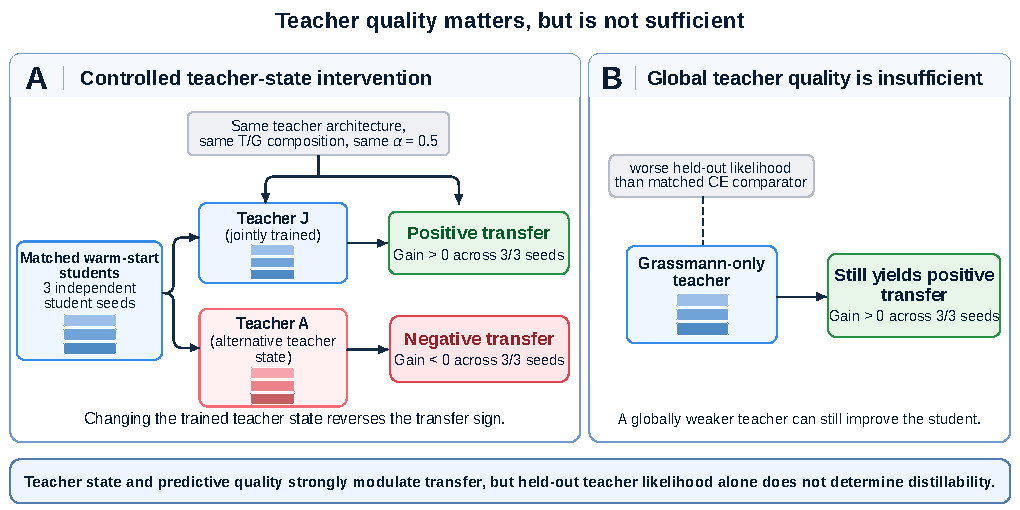
\includegraphics[width=\linewidth]{figures/fig3_teacher_quality.pdf}
\caption{Teacher-state and likelihood controls on WikiText-2. Changing trained teacher state reverses transfer at fixed composition. A weaker Grassmann-only source still transfers positively. Neither control establishes scalar-likelihood causality or a geometry-specific KD advantage.}
\label{fig:teacher_quality}
\end{figure}

\section{Teacher Source, Ensemble, and Diagnostic Controls}
\label{sec:controls}
\writingtodo{Test V2-H2--H4 while retaining quality/parameter/optimization confounds.}
% - E6/C4: fused gains > both branch gains; T-only saturation warning.
% - E7: TT better all3, H=-0.012460 +/-0.001348; teacher quality and count
%   favor TT, alpha LR differs. No intrinsic superiority in either direction.
% - E8/E9: JSD incremental AUROC tiny; larger TG disagreement yet lower gain.
% - E10/Phase3A: 21 dependent seed-level conditions, 7 families, 63 calibration
%   rows. First/second-order signs identical; seed AUROC0.644444,
%   sign accuracy0.571429, stable subsets11/21. Curvature adds no sign split.
% - This is negative diagnostic evidence, not a successful or proposed method.
% TODO[CAVEAT]: original source ranking PARTIAL; no Safe-lambda recommendation.
% TODO[CITE]: du2020agree, stanton2021really, zhou2022metadistil; do not
% refute their adaptive/online methods from our offline predictor failure.
% MUST NOT: heterogeneity superiority, JSD universal mechanism, Pluecker cause.
% Numeric rows formatted from frozen archived tables; caption revised 2026-10-08.
\begin{table}[htbp]
\centering\small
\begin{tabular}{lrrr}
\toprule
Source & $\alpha$ & Teacher val NLL & Gain (mean $\pm$ SD) \\
\midrule
Fused & 0.5 & 4.300646 & 0.155665 $\pm$ 0.007692 \\
Transformer-only & 1.0 & 4.445647 & 0.134868 $\pm$ 0.008906 \\
Grassmann-only & 0.0 & 4.652064 & 0.040991 $\pm$ 0.006733 \\
\bottomrule
\end{tabular}
\caption{Teacher-source ablation on WikiText-2. Teacher NLL uses the archived 512-chunk subset; gain is the three-student test mean with sample SD. Source changes also change predictive quality. Transformer-only retains the clipping warning.}
\label{tab:teacher_sources}
\end{table}

% Generated from frozen sources by build_tables.py; not a prose draft.
\begin{table}[htbp]
\centering\small
\begin{tabular}{lrrrrr}
\toprule
Teacher & Parameters & Val NLL & JSD & Agreement & KD gain \\
\midrule
TG & 37,749,633 & 4.303697 & 0.182087 & 0.507034 & 0.155665 \\
TT & 35,340,801 & 4.293589 & 0.099793 & 0.630170 & 0.168125 \\
\bottomrule
\end{tabular}
\caption{Homogeneous TT control versus heterogeneous TG (planning table).}
\label{tab:tt_vs_tg}
\par\smallskip\begin{minipage}{0.96\linewidth}\footnotesize Common full validation split for teacher metrics. $H=\mathrm{NLL}_{TT}-\mathrm{NLL}_{TG}=-0.012460\pm0.001348$, TT better for 3/3 students. TT is about 6.38\% smaller, has 0.010108 lower teacher NLL, and uses a different alpha learning rate (0.01 versus historical TG 0.005). This rejects a TG superiority claim here, not all heterogeneous ensembles.\end{minipage}
\end{table}

% Generated from frozen sources by build_tables.py; not a prose draft.
\begin{table}[htbp]
\centering\small
\begin{tabular}{lrrrr}
\toprule
Offline predictor & Conditions & AUROC & Sign accuracy & Spearman \\
\midrule
Validation dot a & 21 & 0.644444 & 0.571429 & 0.249351 \\
Quadratic gain & 21 & 0.644444 & 0.571429 & 0.249351 \\
Virtual nominal gain & 21 & 0.700000 & 0.571429 & 0.427273 \\
\bottomrule
\end{tabular}
\caption{Local diagnostics do not reliably predict endpoint transfer (planning table).}
\label{tab:local_diagnostics}
\par\smallskip\begin{minipage}{0.96\linewidth}\footnotesize 21 conditions in seven dependent families; three calibration subsets each, not 63 independent runs. First/second-order signs agree on 63/63 calibration rows, but are calibration-stable for only 11/21 conditions. Curvature adds no sign separation. Negative diagnostic, not a proposed successful Safe-lambda method.\end{minipage}
\end{table}

\figureplaceholder{F4: Homogeneous ensemble control}
{Paired TG/TT gains and a separate teacher-quality/diversity panel. Include
parameter counts, H direction and alpha-learning-rate mismatch.}
{fig:ensemble_control}

\section{A Bounded Modern External-Validity Stress Test}
\label{sec:external-validity}

We examine pretrained SmolLM2-360M teacher supervision of SmolLM2-135M students~\citep{benallal2025smollm2} on a fixed FineWeb-Edu subset~\citep{penedo2024fineweb}. Three independent student adaptations use the same frozen adapted teacher, token splits, and continuation protocol. Relative to matched CE, KD gives mean gains of $-0.013550\pm0.003542$ at $\lambda=1$ and $-0.043924\pm0.004017$ at $\lambda=5$, both negative in all three seeds with agreeing validation and test directions (Table~\ref{tab:modern_stress}). The teacher has substantially better held-out likelihood.

Each preparation and continuation receives the same 10M-target budget. CE and KD begin from identical selected student weights within a seed, and test follows validation selection. These replications vary adaptation of one pretrained student base, not independent pretraining. The comparison therefore concerns the frozen continuation recipe rather than modern KD in general.

Checkpoint eligibility changes the interpretation. When the original $S_0$ is added as a step-0 validation candidate, all nine CE, KD1, and KD5 selections choose $S_0$. This diagnostic leaves primary trained-checkpoint endpoints intact but shows that further CE training is itself unnecessary in this regime. The result is therefore not a clean modern negative-transfer confirmation. The $\lambda=5$ arms retain \texttt{CLIP\_SATURATION\_WARNING}; frequent clipping at $\lambda=1$ remains a limitation, not evidence that clipping causes degradation.

Thus, degradation relative to CE and lack of useful continuation are distinct observations that must be reported together.

A CE-only headroom control starts from a fixed early student and uses a deterministic continuation stream excluding targets already consumed in preparation. Under the preregistered learning-rate candidates and budget, the best validation improvement is only $+0.004849$, below the 0.01 gate. The gate fails, so no conditional KD or new test endpoint is evaluated.

This control asks whether CE can first establish sufficient remaining headroom, not which KD strength yields a preferred outcome. Its small positive validation change does not satisfy the registered requirement.

These modern results are a bounded stress test of continuation and selection, not a primary claim about modern KD. They neither show that better teachers generally harm students nor identify FineWeb-Edu as a cause of negative transfer. Exact selection records, optimization telemetry, pretraining-overlap uncertainty, and the failed gate appear in Appendix~\ref{app:modern}.

% Numeric rows formatted from frozen archived tables; caption revised 2026-10-08.
\begin{table}[htbp]
\centering\small
\begin{tabular}{lrrr}
\toprule
Strength & Mean test gain & Sample SD & Negative signs \\
\midrule
1 & -0.013550 & 0.003542 & 3/3 \\
5 & -0.043924 & 0.004017 & 3/3 \\
\bottomrule
\end{tabular}
\caption{FineWeb-Edu pretrained-model stress test. CE-relative test gains use trained-checkpoint validation selection, excluding $S_0$. Both strengths have 3/3 negative signs. When step 0 is separately admitted, all nine arms select $S_0$; this is not clean modern negative-transfer confirmation.}
\label{tab:modern_stress}
\end{table}


\section{Discussion and Limitations}\label{sec:discussion}
\writingtodo{Synthesize configuration dependence without a causal theorem.}
% - Evidence is consistent with joint teacher state, student state and
%   optimization-configuration dependence, not a fully factorial decomposition.
% - Three student seeds, shared WT2 S0/C0, one teacher/corpus; adaptation versus
%   pretraining independence; calibration tokens/subsets not extra run units.
% - Teacher-quality and alpha-LR/parameter-count confounds; persistent/frequent
%   clipping, AMP event rates, selection eligibility, failed gates/amendments.
% - Phase4C gate failure unresolved; modern external validity limited.
% - ATKD/other adaptive baselines not run; literature overlap already substantial.
% TODO[LIMITATIONS]: preserve every warning in V2 registry and original reports.
% - Deployment is secondary; batch1 quality-student slower than teacher;
%   no blanket speedup or geometric efficiency attribution.
% MUST NOT: universal scalar predictor, general KD failure or causal geometry.

\section{Conclusion}\label{sec:conclusion}
\writingtodo{Summarize only C1--C4 and their bounded configuration-level implication.}
% - Reproducible +/+/- outcomes; fixed-composition teacher-state modulation;
%   scalar quality insufficiency; ensemble gains without TG superiority.
% - Secondary diagnostics/stress test constrain, not enlarge, mechanism claims.
% MUST NOT: new evidence, new proposed method, automatic experiments or a
% theorem that distillability is fully explained by measured configuration axes.

\clearpage
\bibliographystyle{plainnat}
\begingroup\raggedright
\bibliography{references}
\endgroup
\clearpage
\appendix
\setcounter{figure}{0}
\renewcommand{\thefigure}{A\arabic{figure}}
\renewcommand{\theHfigure}{appendix.\arabic{figure}}
\section{Grassmann and Test-Bed Details}\label{app:architecture}
\writingtodo{Add verified architecture equations and dimensions as test-bed context.}
% - Preserve actual feature-dependent gates; distinguish branch models from
%   late-logit scalar alpha composition. Do not recycle inaccurate old claims.
% TODO[VERIFY_EXTERNAL]: primary Grassmann/Pluecker background references.
% MUST NOT: mathematical detail as evidence of geometric KD superiority.

\section{Full Protocols and Amendments}\label{app:protocols}
\writingtodo{Transcribe exact frozen per-domain protocols, hashes and amendments.}
% - Original Phase2D failed short A smoke; explicitly amended matched full-data
%   gate; Phase2E authorized unchanged T saturation; FP16 AMP maxima nonzero.
% - Teacher val subset vs full-split scope, validation-selected endpoints,
%   per-domain budgets, S0 independent training, teacher identity and hashes.
% - Modern protocol/reset/order/BF16 and step0 eligibility differ from Phase2.

\section{Per-Seed Endpoint Tables}\label{app:per-seed}
\writingtodo{Insert exact per-seed tables from the V2 source inventory.}
% - research/manuscript_v2/tables/table_endpoint_inventory.csv; original
%   Phase2C/2D/2E/2F/2G CSVs; PTB legacy-rounded PPL is not an exact NLL source.
% - Same WT2 seeds reused across controls; no independent-condition inflation.

\section{Branch Disagreement Details}\label{app:branch-diagnostics}
\writingtodo{Insert token-level JSD analysis with its observational limits.}
% - Incremental AUROC PTB-0.000323/TS+0.010910; R2+0.000533/+0.003061.
% - One endpoint pair per dataset; token bootstrap not model-seed replication.

\section{Local Gradient and Curvature Diagnostics}\label{app:local-diagnostics}
\writingtodo{Reuse Phase3A tables/figures with failed-diagnostic scope.}
% - Seven families/21 dependent conditions/63 calibration rows; calibration
%   instability, first/second same signs, curvature0.52% median correction.
% - Literal first LR0 no-op; candidate safe lambdas not recommendations.

\section{Modern Selection and Optimization Details}\label{app:modern}
\writingtodo{Insert Phase4A--4C records and permanent warnings.}
% - Modern TinyStories pilot42 unreplicated, distinct from Phase2G confirmation.
% - All9/9 best_including_S0 choices; CE deterioration; adapted not pretrained
%   seed independence; original primary trained-step comparisons unchanged.
% - CLIP_SATURATION_WARNING, frequent L1 clipping, CE456 finite86.482155
%   spike and Phase4C2e-5 finite14.602655 spike; causes/impacts UNKNOWN.
% - Gate fails at0.004849292809; no conditional KD or new test/ratio measurements.

\section{Failed and Legacy Controls}\label{app:failed-controls}
\writingtodo{Keep failed CRBD, shuffle, legacy CodeParrot and unmatched RI separate.}
% - CRBD20k one seed: CE5.0195/fixedKD5.3018/CRBD5.5067/shuffle5.5010 PPL;
%   all KD clip-saturated; repair-0.7220. Not a successful method contribution.
% - Legacy CodeParrot common5k gain+0.188309, old loss/single-seed/winner-selection.
% - Random-init learning rates/budgets unmatched: no warm-start necessity.

\section{Legacy Efficiency and Deployment Trade-offs}\label{app:efficiency}
\writingtodo{Insert frozen PTB deployment observations with scope labels.}
% - Historical configs36.264305/31.434257/23.565121M, not current TT/TG counts.
% - Batch32 latency55.984/48.460/34.959ms, RTX3090 seq256, single checkpoint;
%   batch1 quality16.089ms >teacher15.482ms, so no universal inference speedup.
% - Frozen table_efficiency.csv is separate from confirmatory matched KD gains.

\end{document}
